
As introduced in section \ref{section:Introduction}, SmartEater \footnote{\url{https://sites.google.com/site/eatingandanxietylab/resources/smarteater}} will be a mHealth (mobile health) app, that predicts future eating crises based on the user's past behaviour. The predictions are made on smartphone sensor and usage data, therefore reducing strenuous user input. The app will give the user content-dependent feedback, to avert a food craving episode. 

\textcite{AboutToEat2016Rahman} introduced a similar idea in their paper. Their goal was to predict "About-to-Eat" and "Time until the Next Eating Event" stages by using wearable sensing devices, in order to reduce serious health issues (e.g. obesity). The authors state, that detecting when a person is eating is not helpful. It is more beneficial to predict moments shortly before the user is about to eat ("About-To-Eat").

Rahman et al. investigated how people were currently tracking their meals by conducting a survey. Under half of the participants had previously used food tracking/journalling tools. 48.9\% of these stopped using them within the first month. Respondents also  wished for the app to take action directly before a meal/snack ("About-to-Eat" moments), thus supporting the authors' previous assumptions.

The authors used a variety of different sensors to record the following data: physical movement (raw accelerometer, gyroscope, step count, speed), caloric expenditure, heart rate, skin temperature, electrodermal activity (good indicator for psychological arousal), chewing and swallowing sounds (for detection of current eating events) and GPS location. Furthermore, the test subjects recorded self-reports, such as when they started eating, emotional state when eating, intensity of desire/craving and hunger, and end of eating. Eight participants, aged 26-54, participated in this study for five days. The recorded data then underwent cleaning and preprocessing, feature extraction, feature selection and machine learning. 
In the feature extraction step, two parameters were used on the processed sensor time series to create windows. Firstly, the feature extraction window size parameter regulated the time duration in a specific window. While a short window duration could catch immediate characteristics in the sensor time series, a coarse one could be used for long term trends. The authors used a variety of window sizes, varying from 5 to 120 minutes. The prediction model results would decide the best window. The second parameter, the window shift size, established the time duration between two neighbouring windows, for example meaning window \textit{n} is shifted one minute compared to window \textit{(n - 1)}. A constant shift of one minute was used for all window sizes. 

In the feature selection step, the most relevant features were selected (e.g. the location features were not beneficial and merely represented noise). Signal processing and machine learning were used on the sensor streams to train an "About-to-Eat" moment classifier. The classifier's performance was further inspected, in order to see how the different feature extraction window sizes affected it. The small window sizes were vulnerable to noise and the coarser ones were unable to detect recent events, which were crucial in creating the classifier. As can be seen in figure \ref{figure:windowSize}, the smaller window sizes have a higher gap between precision and recall. The performance with window sizes between 60 and 80 minutes is higher and more consistent.

\begin{figure*}[h]
  \centering
  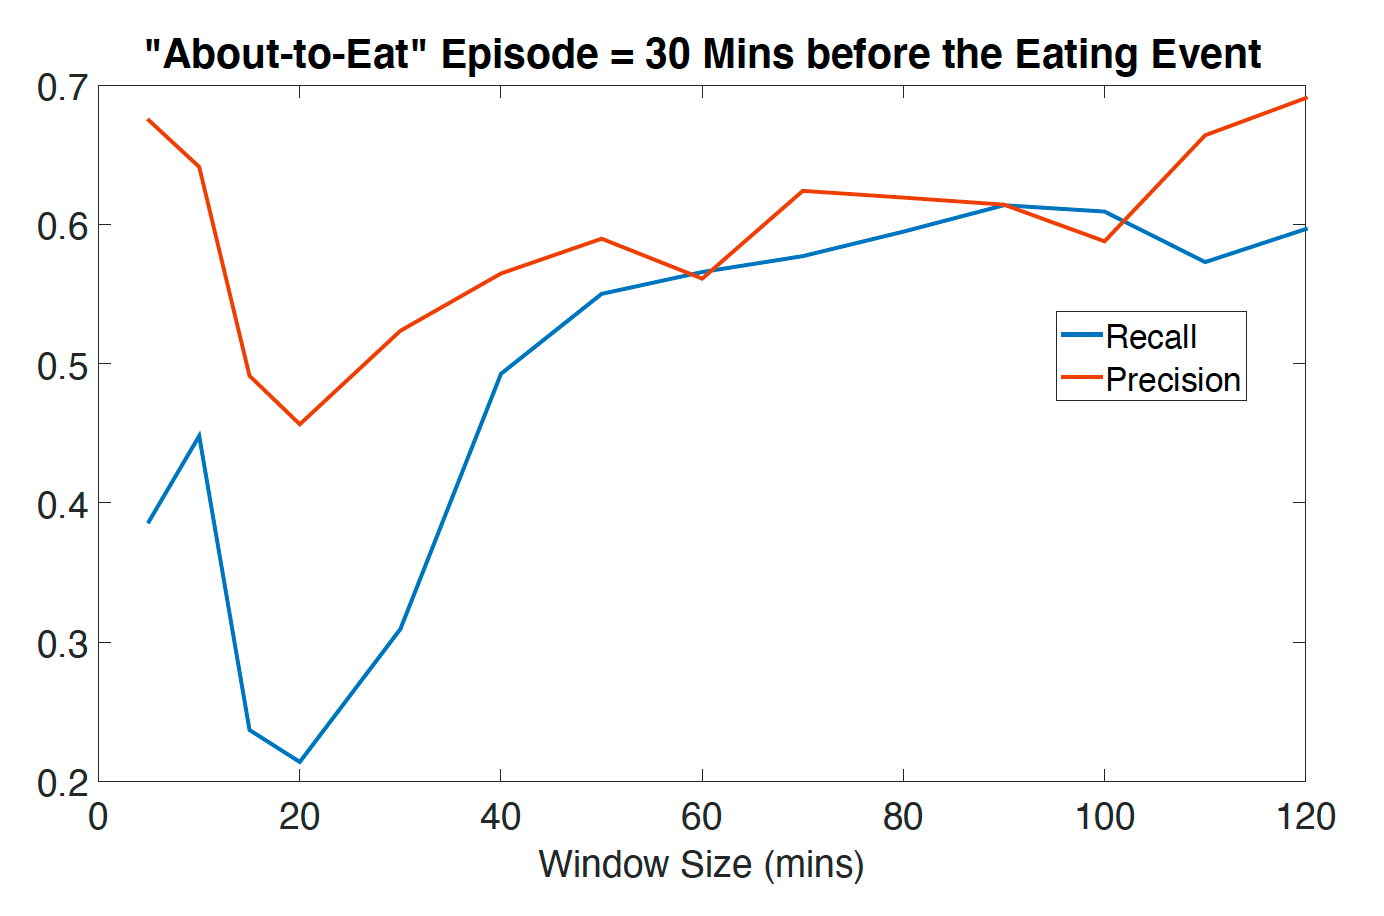
\includegraphics[width=0.5\textwidth]{./images/windowSizePerformance.png}
  \caption{This graph depicts the F measure with the different feature extraction window sizes of the "About-to-Eat" classifier \autocite{AboutToEat2016Rahman}[148]. According to \textcite{han2011data}[306-307], precision and recall are measures used in classification. Precision describes the exactness (how many of the as positive selected items are positive), recall defines the completeness (how many positive items have been correctly selected). The F-score is a measure that combines precision and recall (harmonic mean).}
  \label{figure:windowSize}
\end{figure*}

The performance for the "Time until Next Eating Event" model gained a correlation coefficient of 0.49. The most fitting feature extraction window size was assessed, the best performance was reached with a window size of 100 minutes. The authors further claim, that both models could be improved by incorporating person-dependent data from the target user to the models (e.g. person-specific eating pattern, lifestyle).

\textcite{SmartphoneBasedStressPrediction2015}[240, 242-249] research, whether data collected by a user's smartphone can be used to predict stress. In their study, they used an android smartphone app called "TheStressCollector" (TSC) to collect smartphone usage and sensor data in the background. Collected data included: activity, app usage, network traffic, reboot activity (power on and off events), calls (min, max and mean dB-values collected by the microphone), environment brightness, timestamps of received messages, noise exposure, and screen activity. Fifteen participants installed the app on their smartphone and took part in the conducted study for two weeks. Seven times a day they would fill out questionnaires (at set times), which included the perceived stress score (PSS) and their current stress status. The stress levels were predicted by WEKA's machine learning algorithms. The mean absolute error (MAE) and Pearson correlation were used for the evaluation. The results of this study presented compelling correlations between PSS and the data collected by the smartphone app. The weekly PSS average, as opposed to the daily one, included the highest correlation coefficient. Thus, it is expected, that it is easier to spot longer periods of high stress than shorter ones. This paper is also a team publication featured in the research project from which SmartEater was developed.

In their experiment, \textcite{ClusterPassivelySensedData2018} intend to predict user's negative affect states, in order to provide targeted just-in-time mental health interventions. Sixty-five students participated in the study. Through a smartphone app, GPS location data, accelerometer (activity) data, phone calls, SMS, and ecological momentary assessments (EMA), data was collected and used to cluster participants according to their behavioural profiles. Grouping the participants this way seemed to improve the predictive model's performance.

Other related work: 
\textcite{pius2018automatic} use the k-means clustering algorithm to create automatic annotation of unlabelled smartphone sensor data, to observe sensitive location information of mobile crowd sensing users. \textcite{alcoholCravingPrediction} use smartphone sensor data (e.g. accelerometer) to predict excessive alcohol consumption, in order to replace breathalysers. Their algorithm produced 100\% accuracy, however with 15 minute lags.
